\newpage
\section{実験結果}
選定したシナリオ 28 例中,24例の自律移動を確認した.
以下は1例として \figref{fig:exp_path}に示した Scenario35 を走行時の実験の様子を示す.

\begin{figure*}[htbp]
    \begin{tabular}{ccc}
        \begin{minipage}[t]{0.5\textwidth}
            \centering
            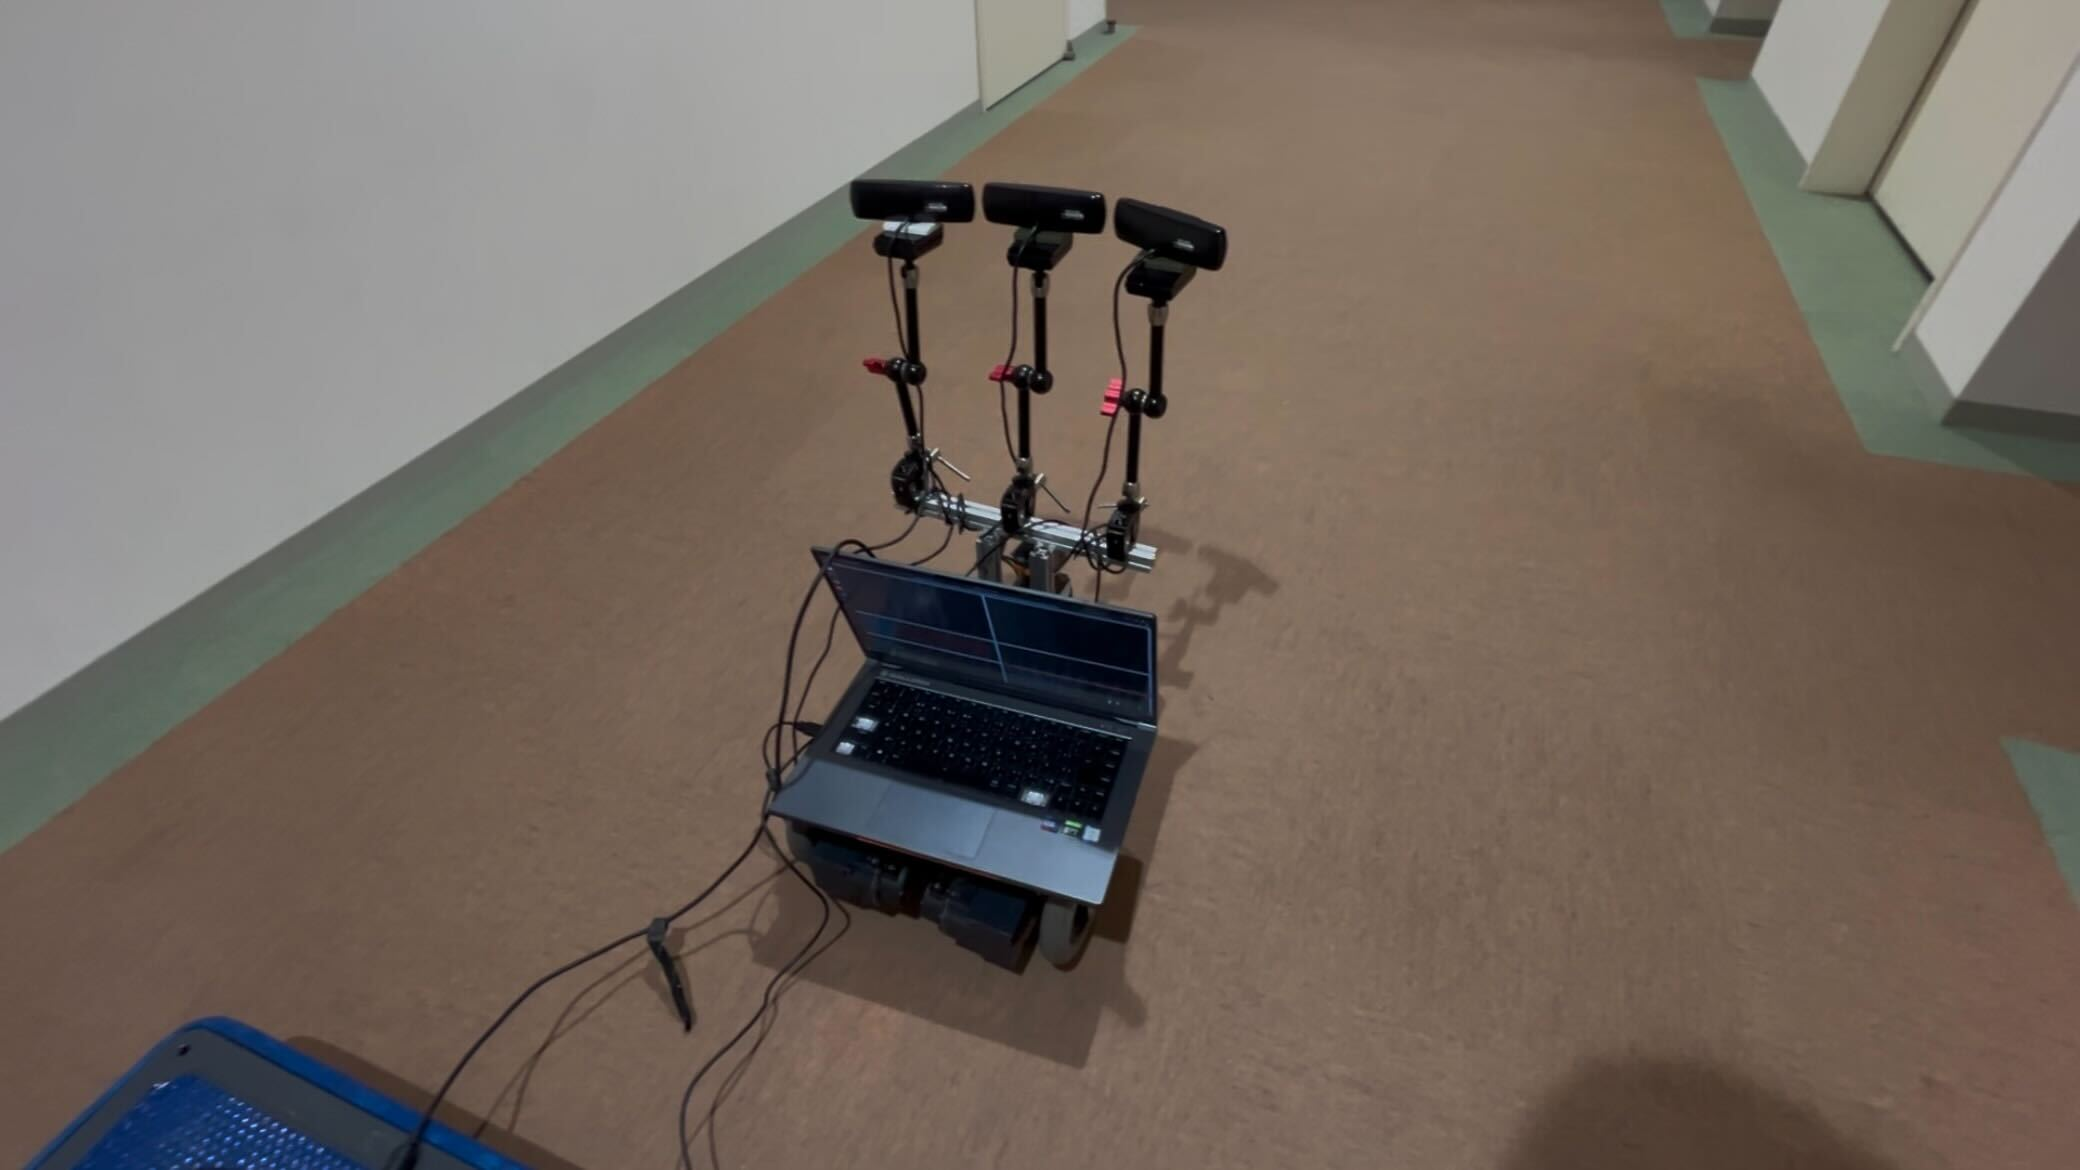
\includegraphics[keepaspectratio, width=70mm]{images/png/ishiguro/exp_0.png}
        \end{minipage} &
        \begin{minipage}[t]{0.5\textwidth}
            \centering
            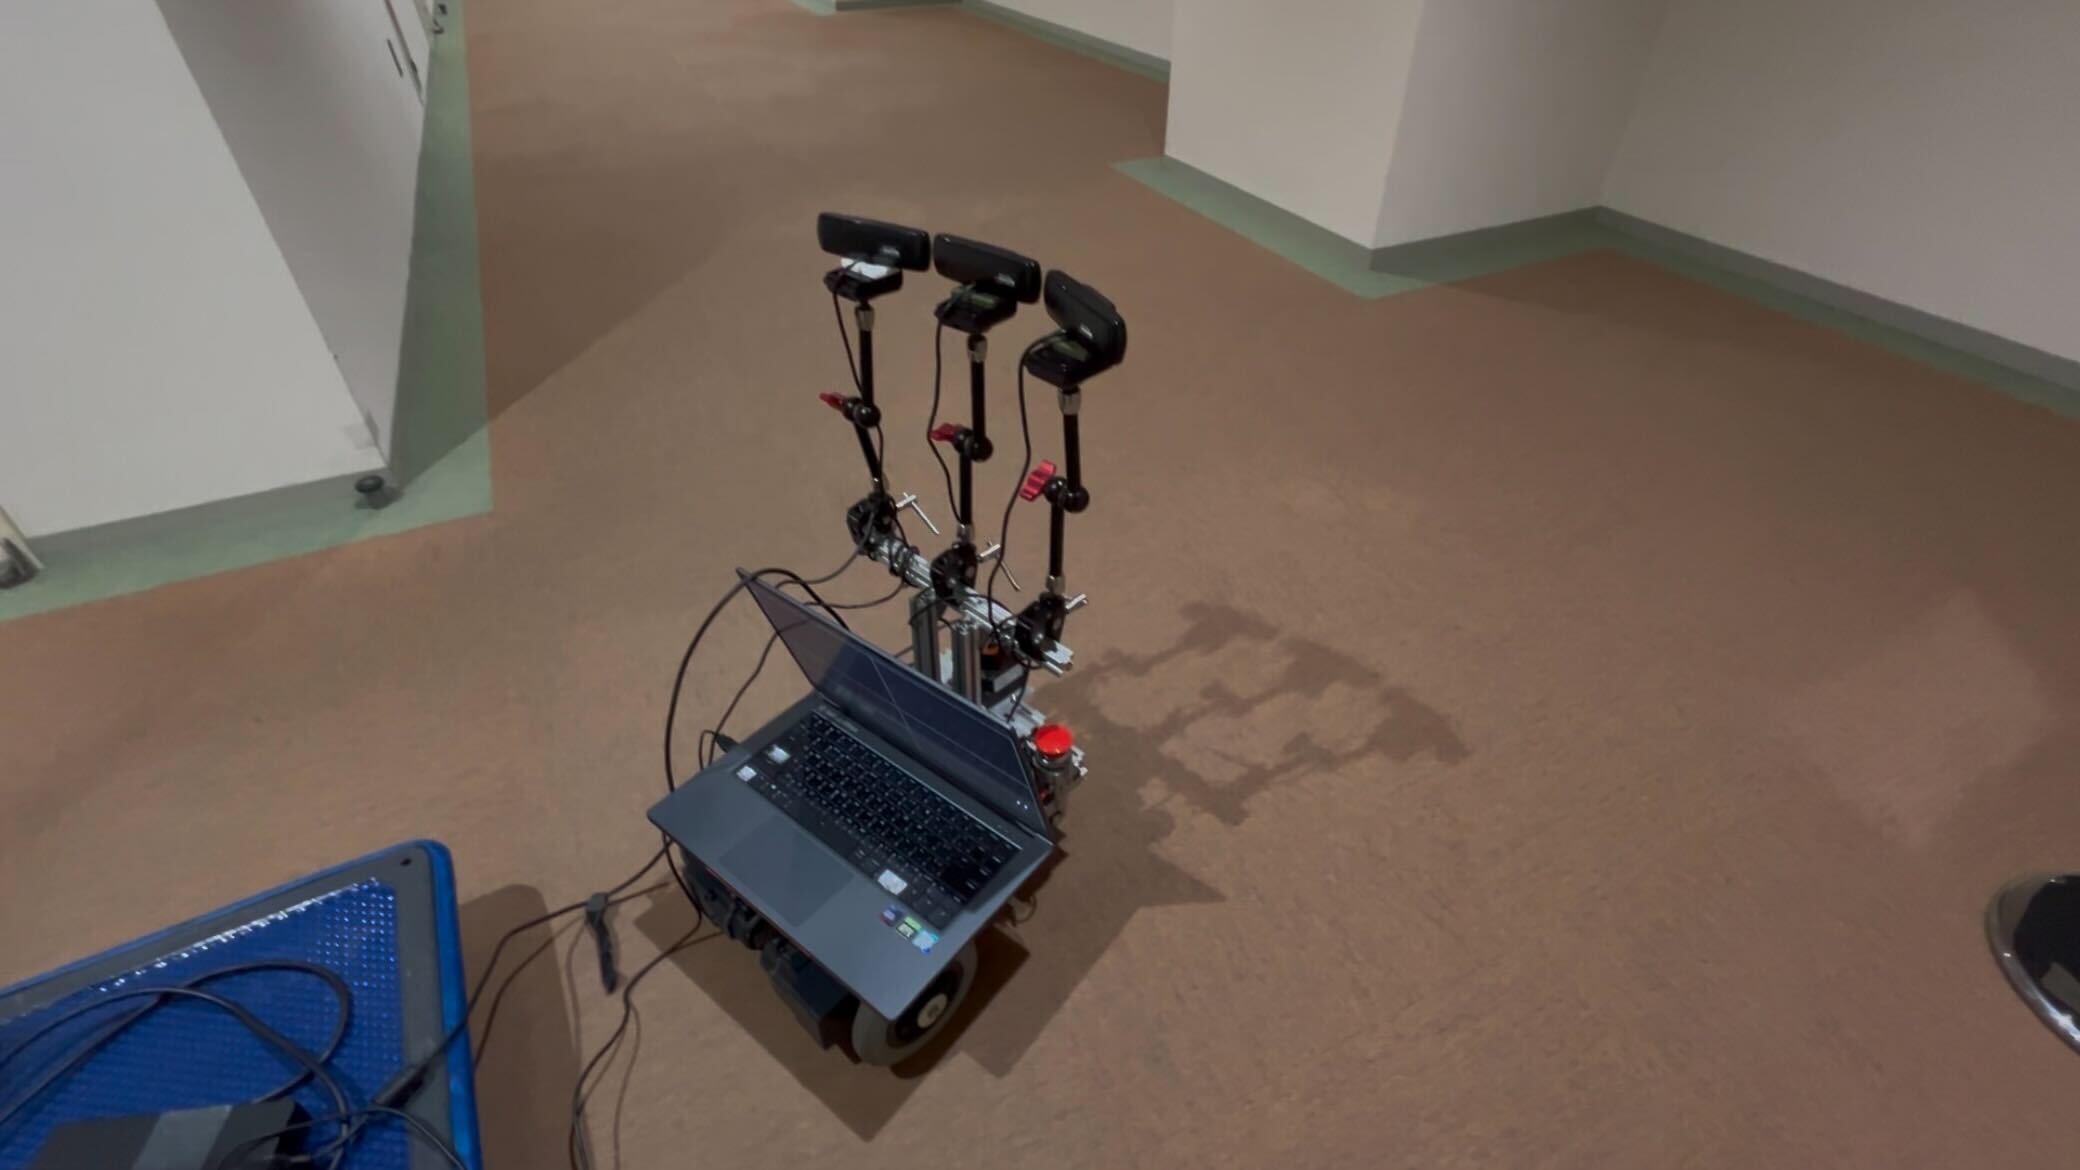
\includegraphics[keepaspectratio, width=70mm]{images/png/ishiguro/exp_1.png}
        \end{minipage} \\
        \begin{minipage}[t]{0.5\textwidth}
            \centering
            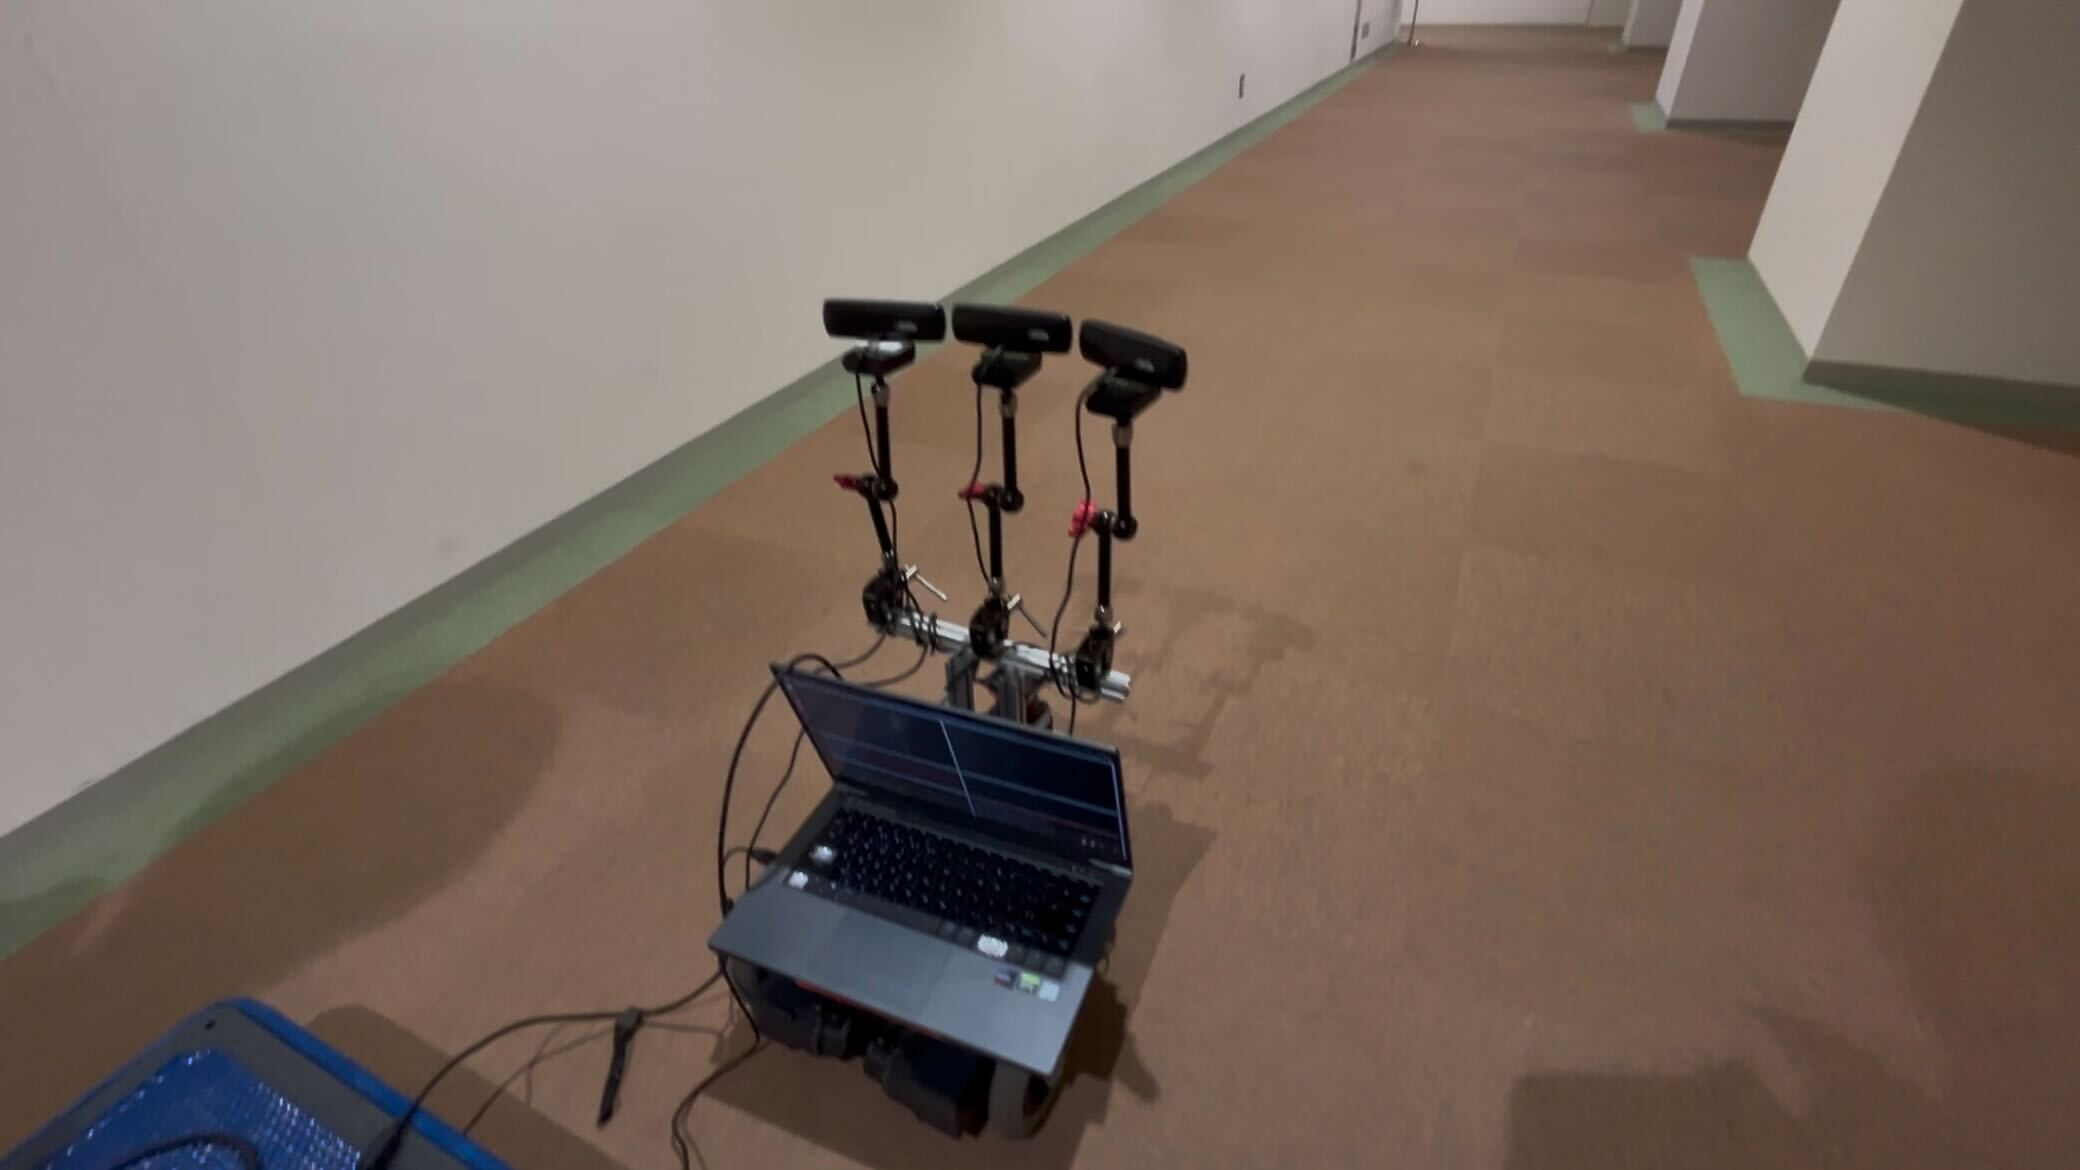
\includegraphics[keepaspectratio, width=70mm]{images/png/ishiguro/exp_2.png}
          % \subcaption{右折(Third 3-way)}
        \end{minipage} &
        \begin{minipage}[t]{0.5\textwidth}
            \centering
            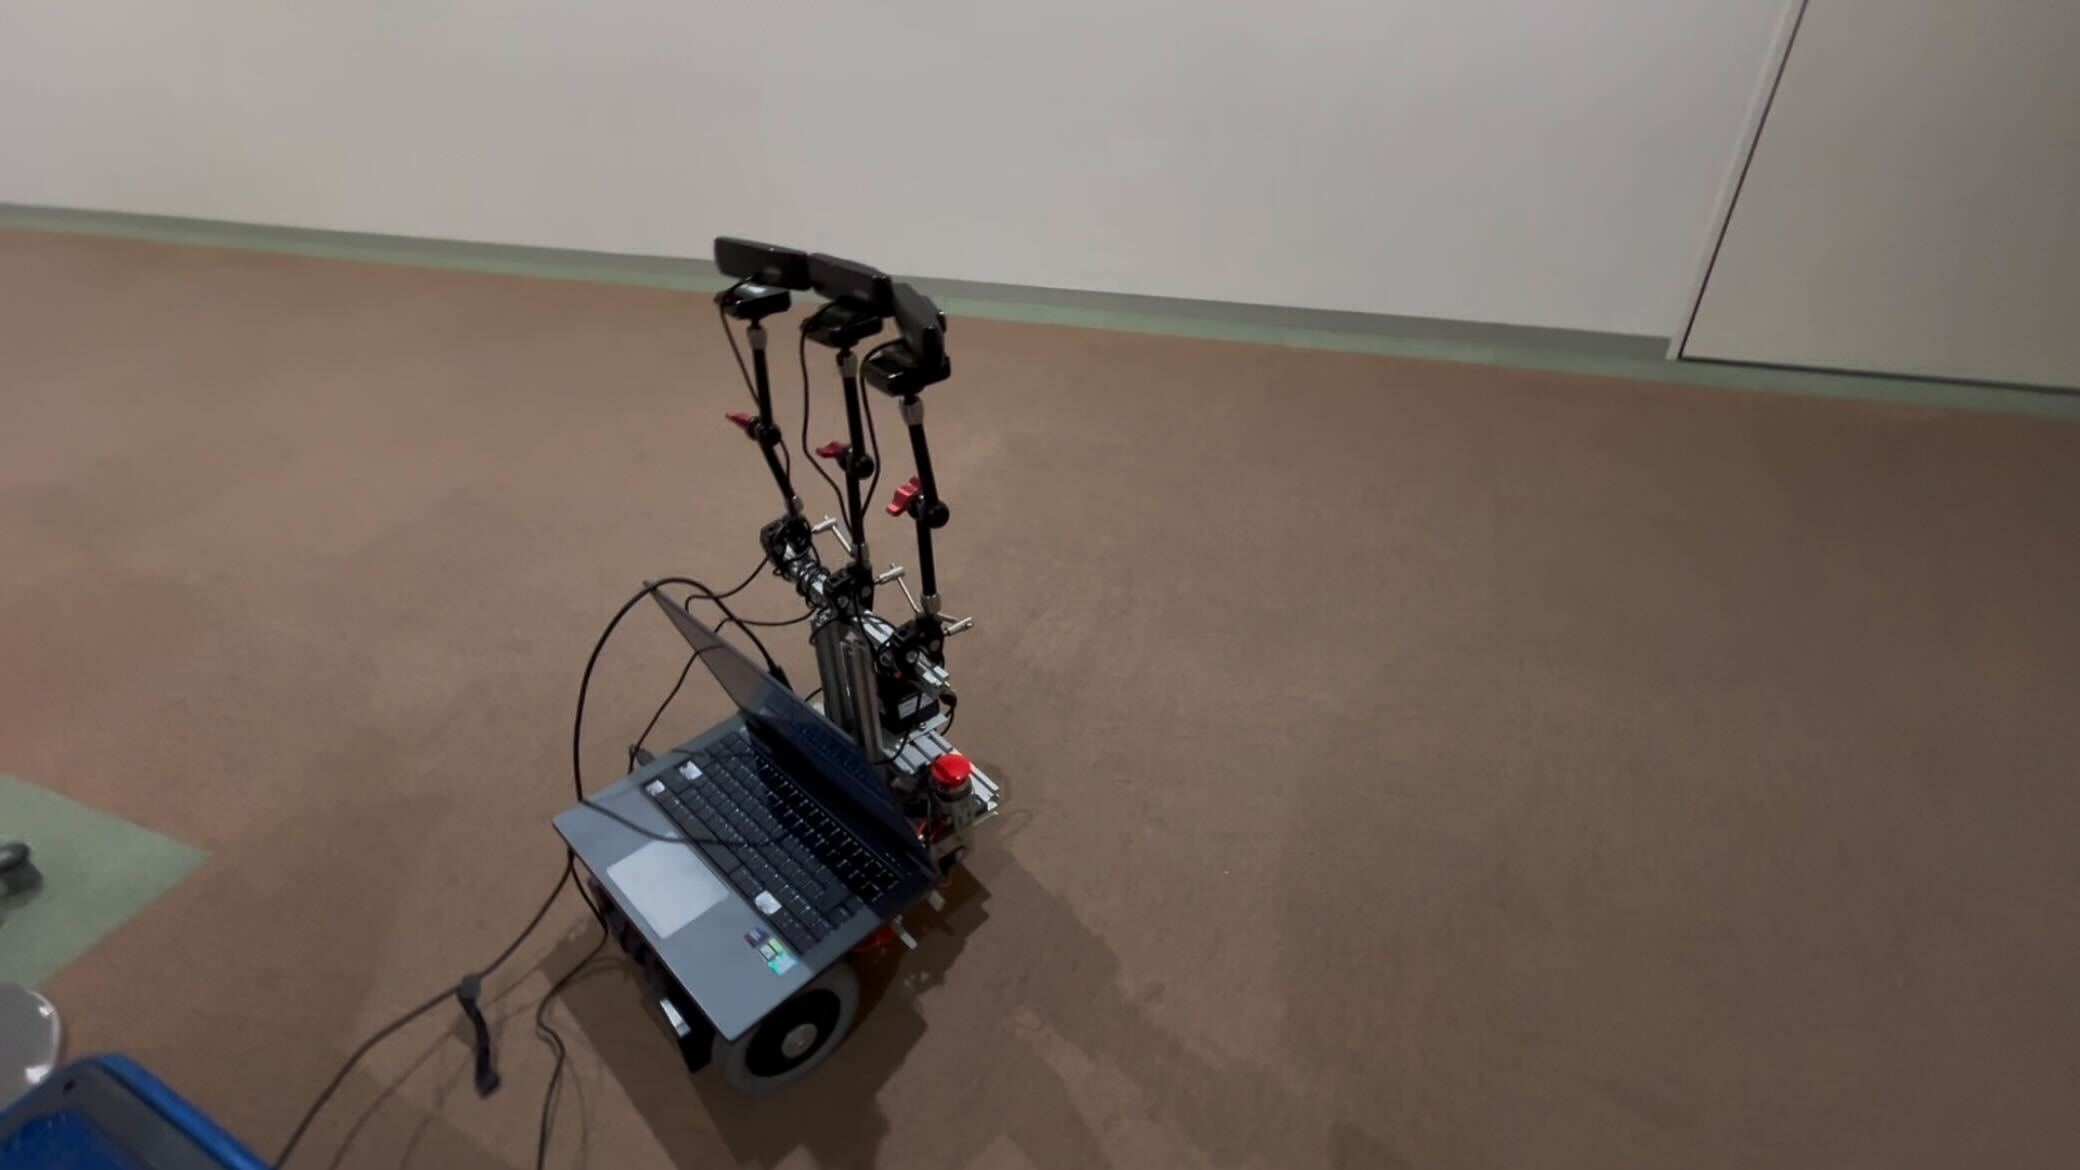
\includegraphics[keepaspectratio, width=70mm]{images/png/ishiguro/exp_3.png}
          % \subcaption{突き当たりまで直進(Straight road)}
        \end{minipage} \\
        \begin{minipage}[t]{0.5\textwidth}
            \centering
            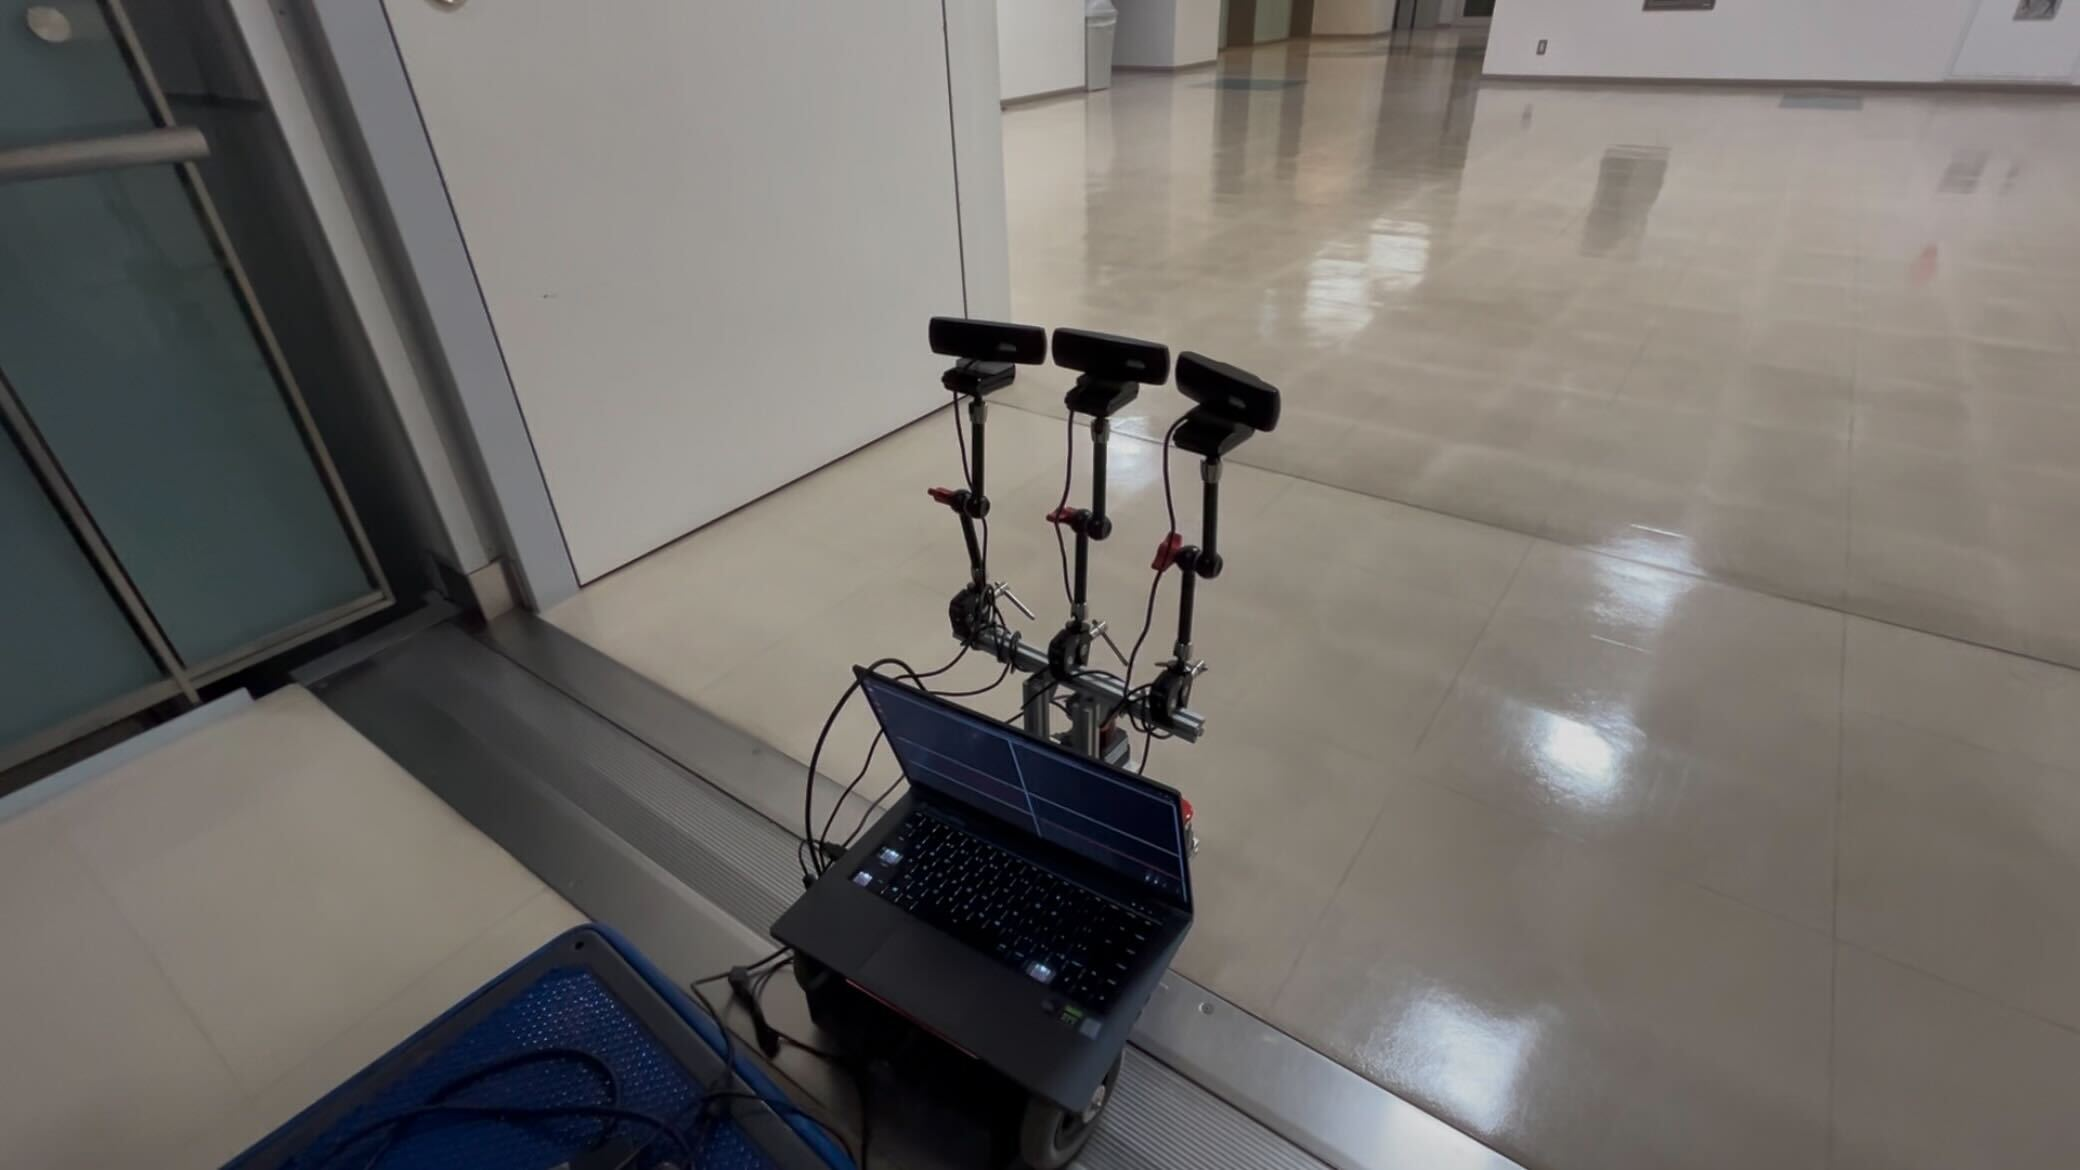
\includegraphics[keepaspectratio, width=70mm]{images/png/ishiguro/exp_4.png}
          % \subcaption{左折(End)}
        \end{minipage} &
        \begin{minipage}[t]{0.5\textwidth}
            \centering
            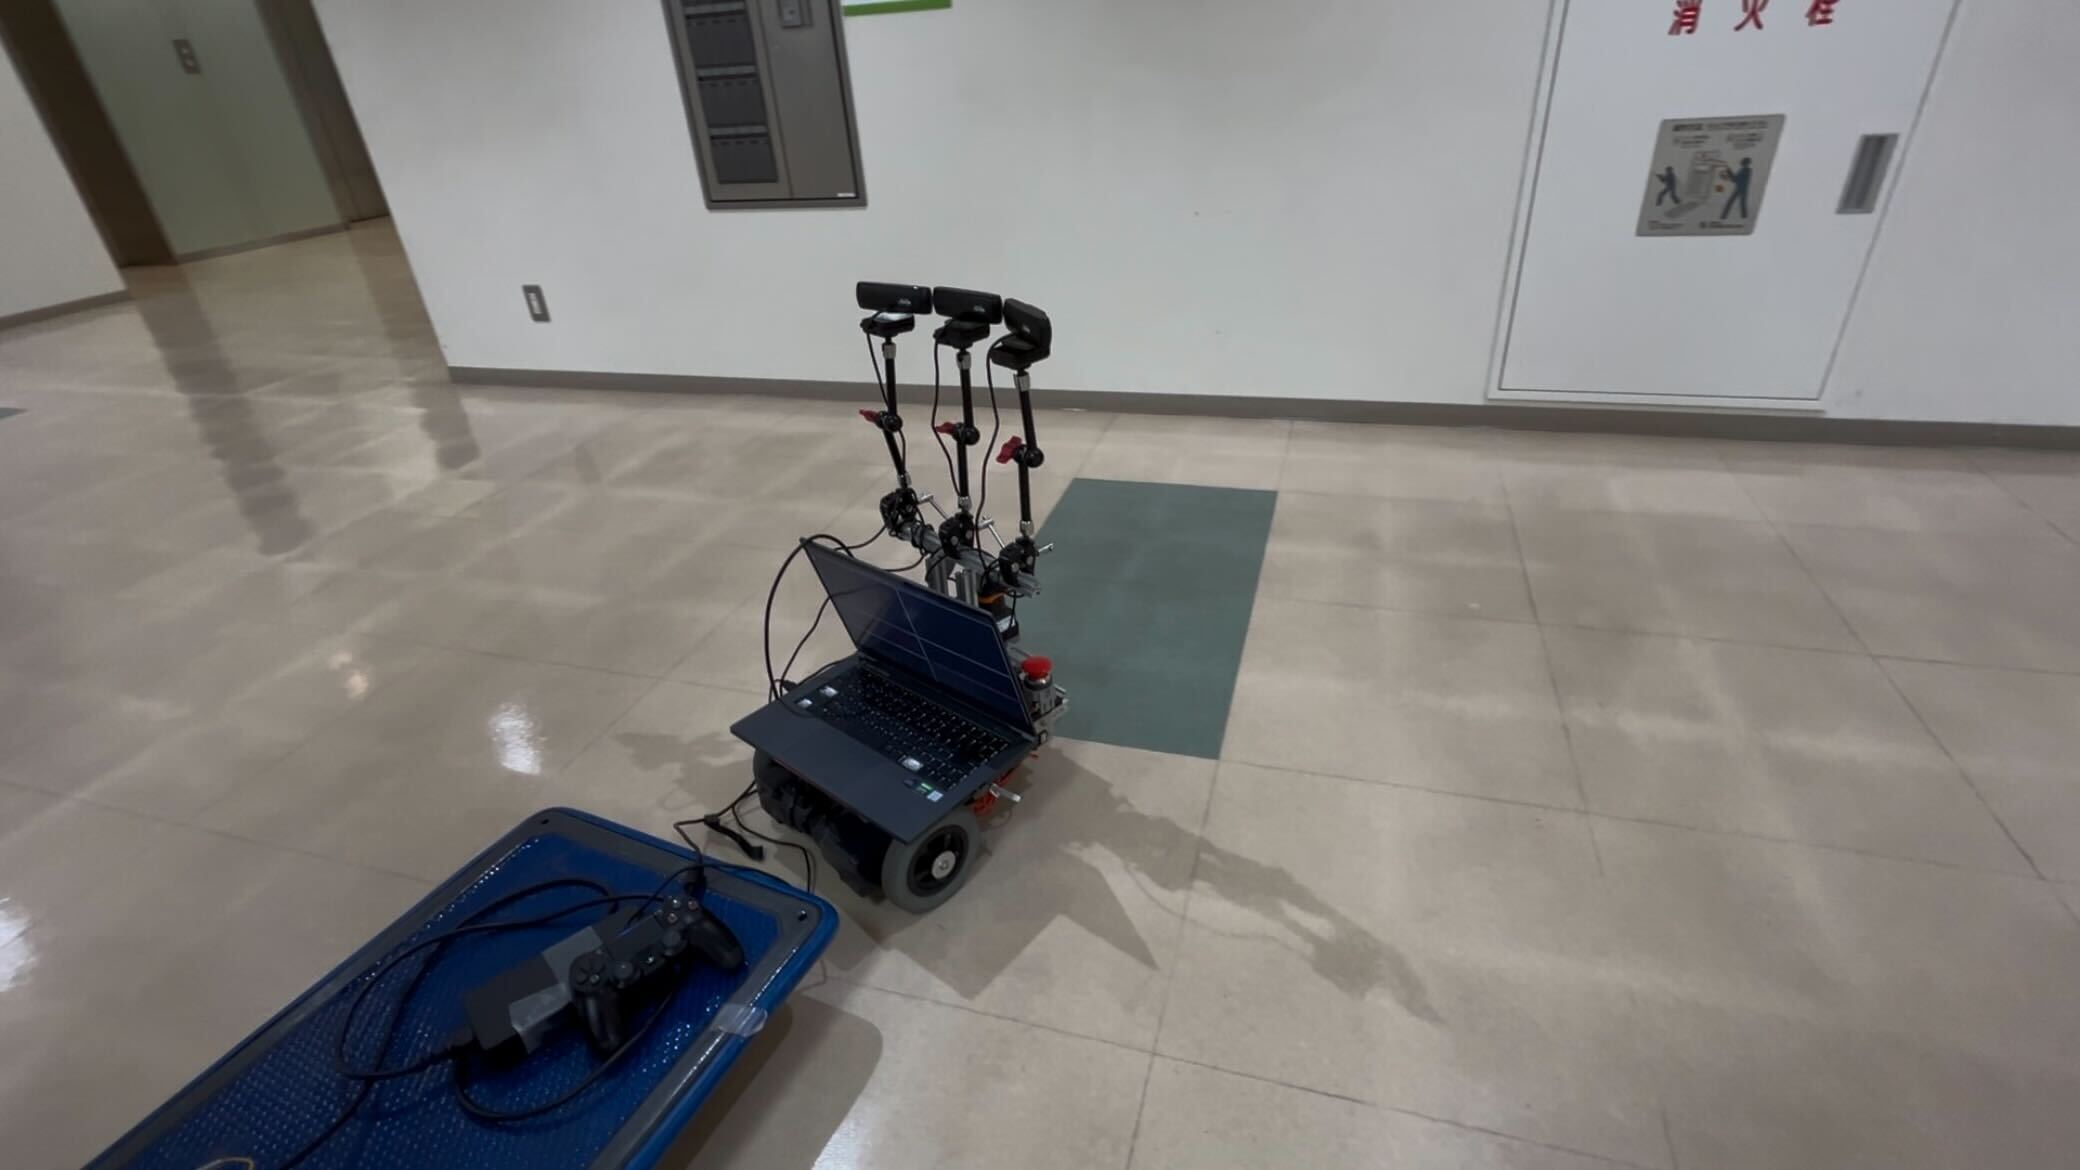
\includegraphics[keepaspectratio, width=70mm]{images/png/ishiguro/exp_5.png}
          % \subcaption{突き当たりまで直進(Straight road)}
        \end{minipage} \\
        \begin{minipage}[t]{0.5\textwidth}
            \centering
            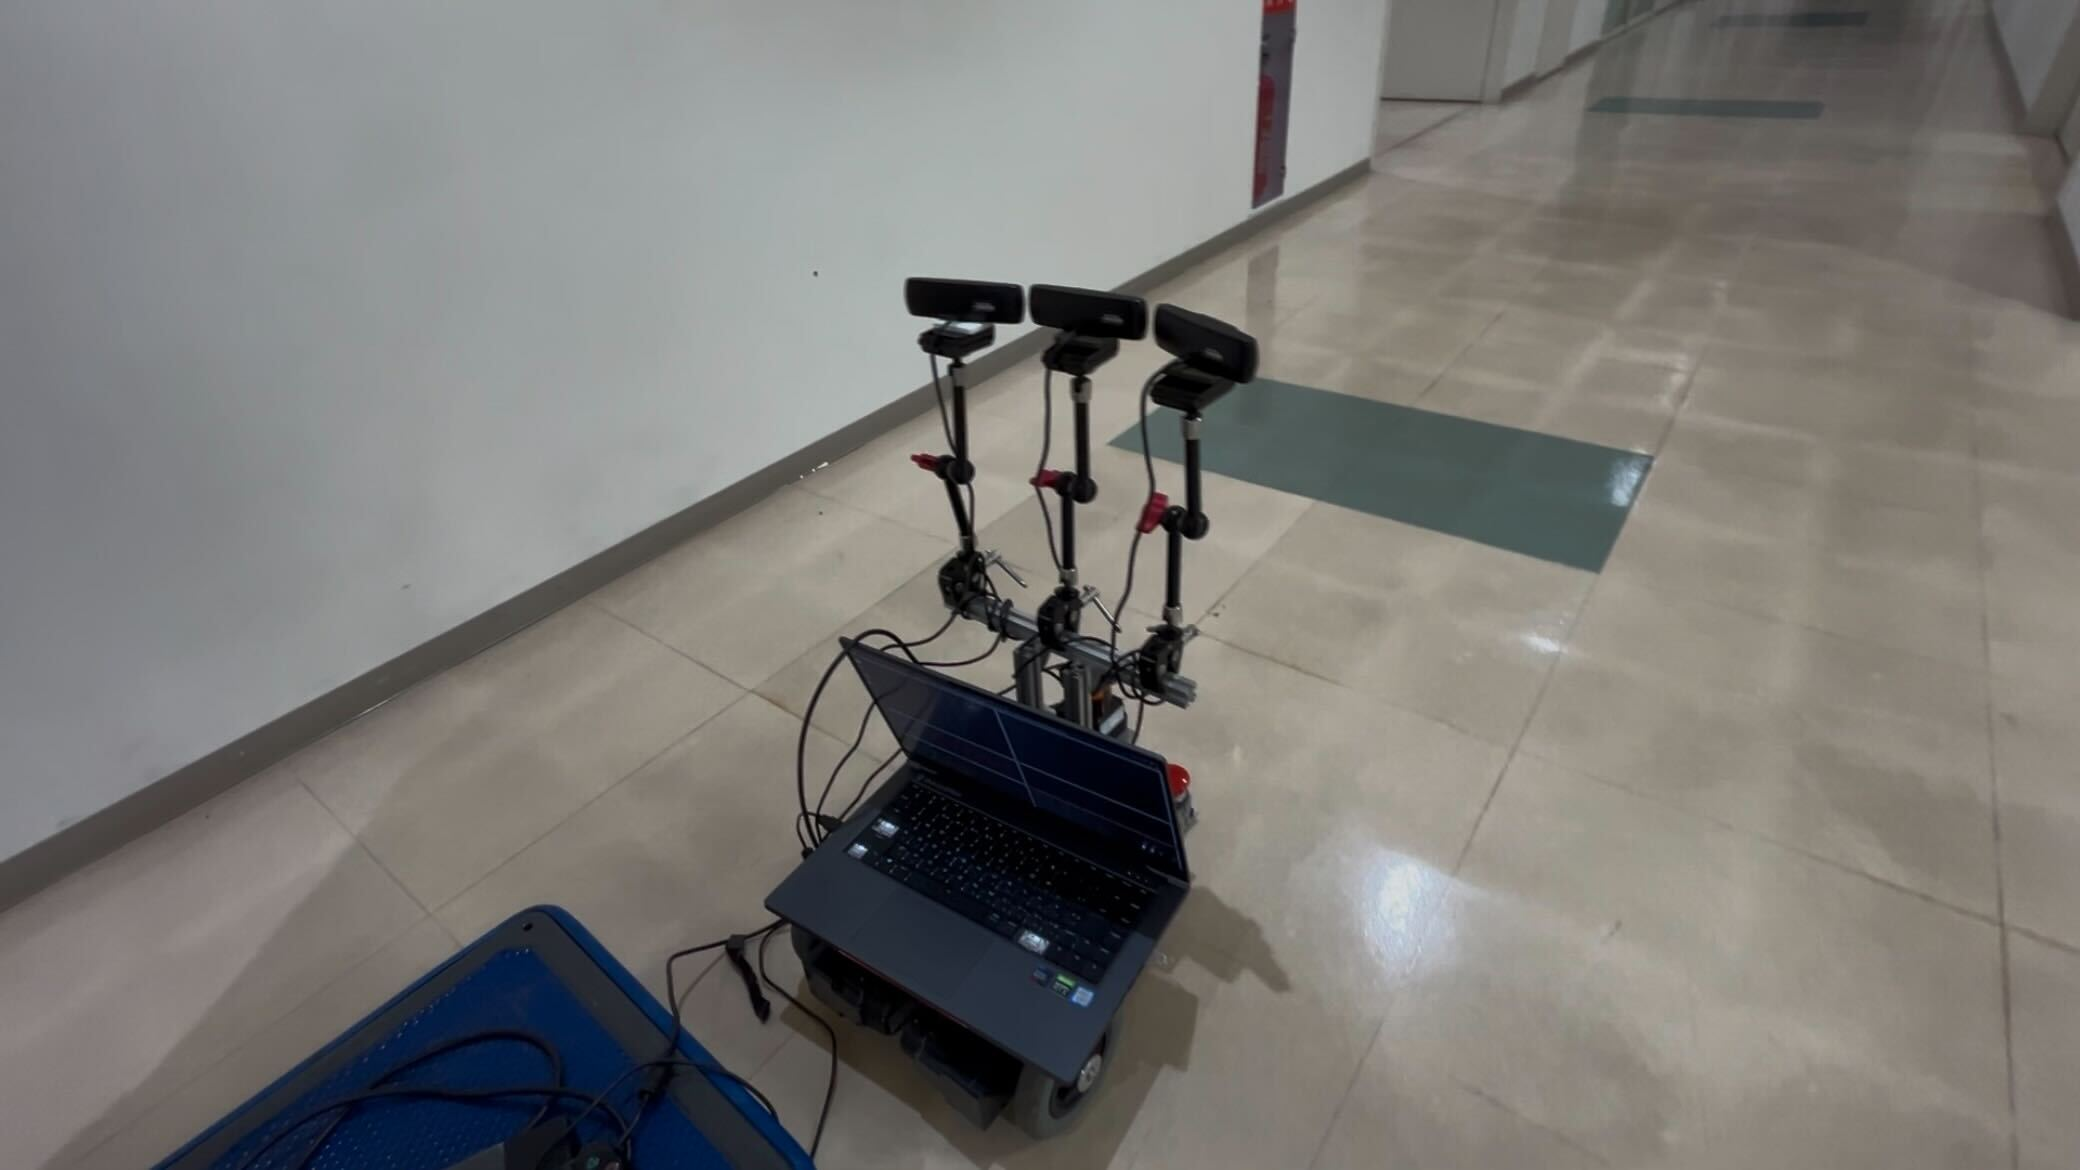
\includegraphics[keepaspectratio, width=70mm]{images/png/ishiguro/exp_6.png}
          % \subcaption{停止(End)}
        \end{minipage} &
        \begin{minipage}[t]{0.5\textwidth}
            \centering
            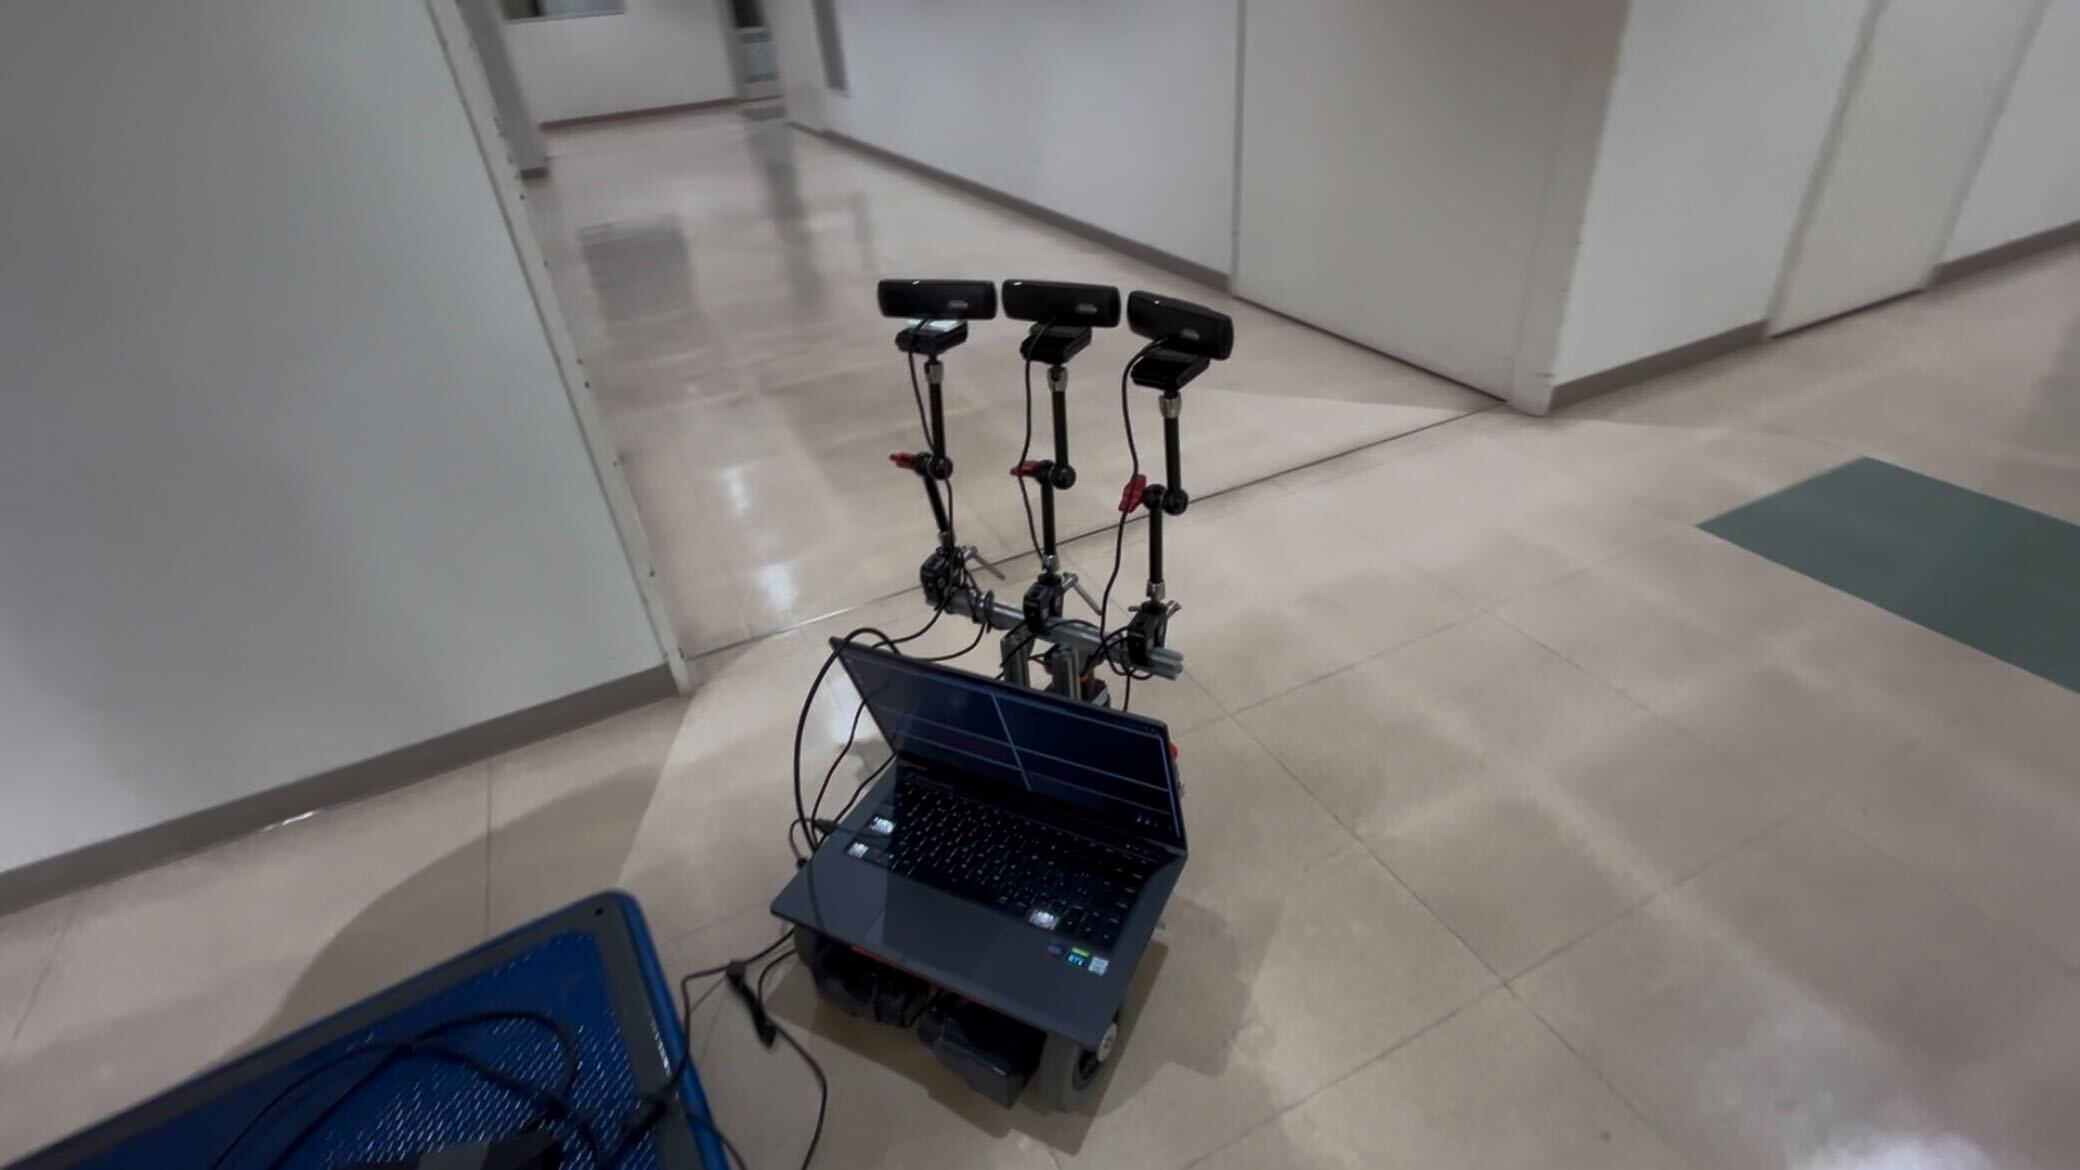
\includegraphics[keepaspectratio, width=70mm]{images/png/ishiguro/exp_7.png}
        % \subcaption{停止(End)}
        \end{minipage} \\
        \begin{minipage}[t]{0.5\textwidth}
            \centering
            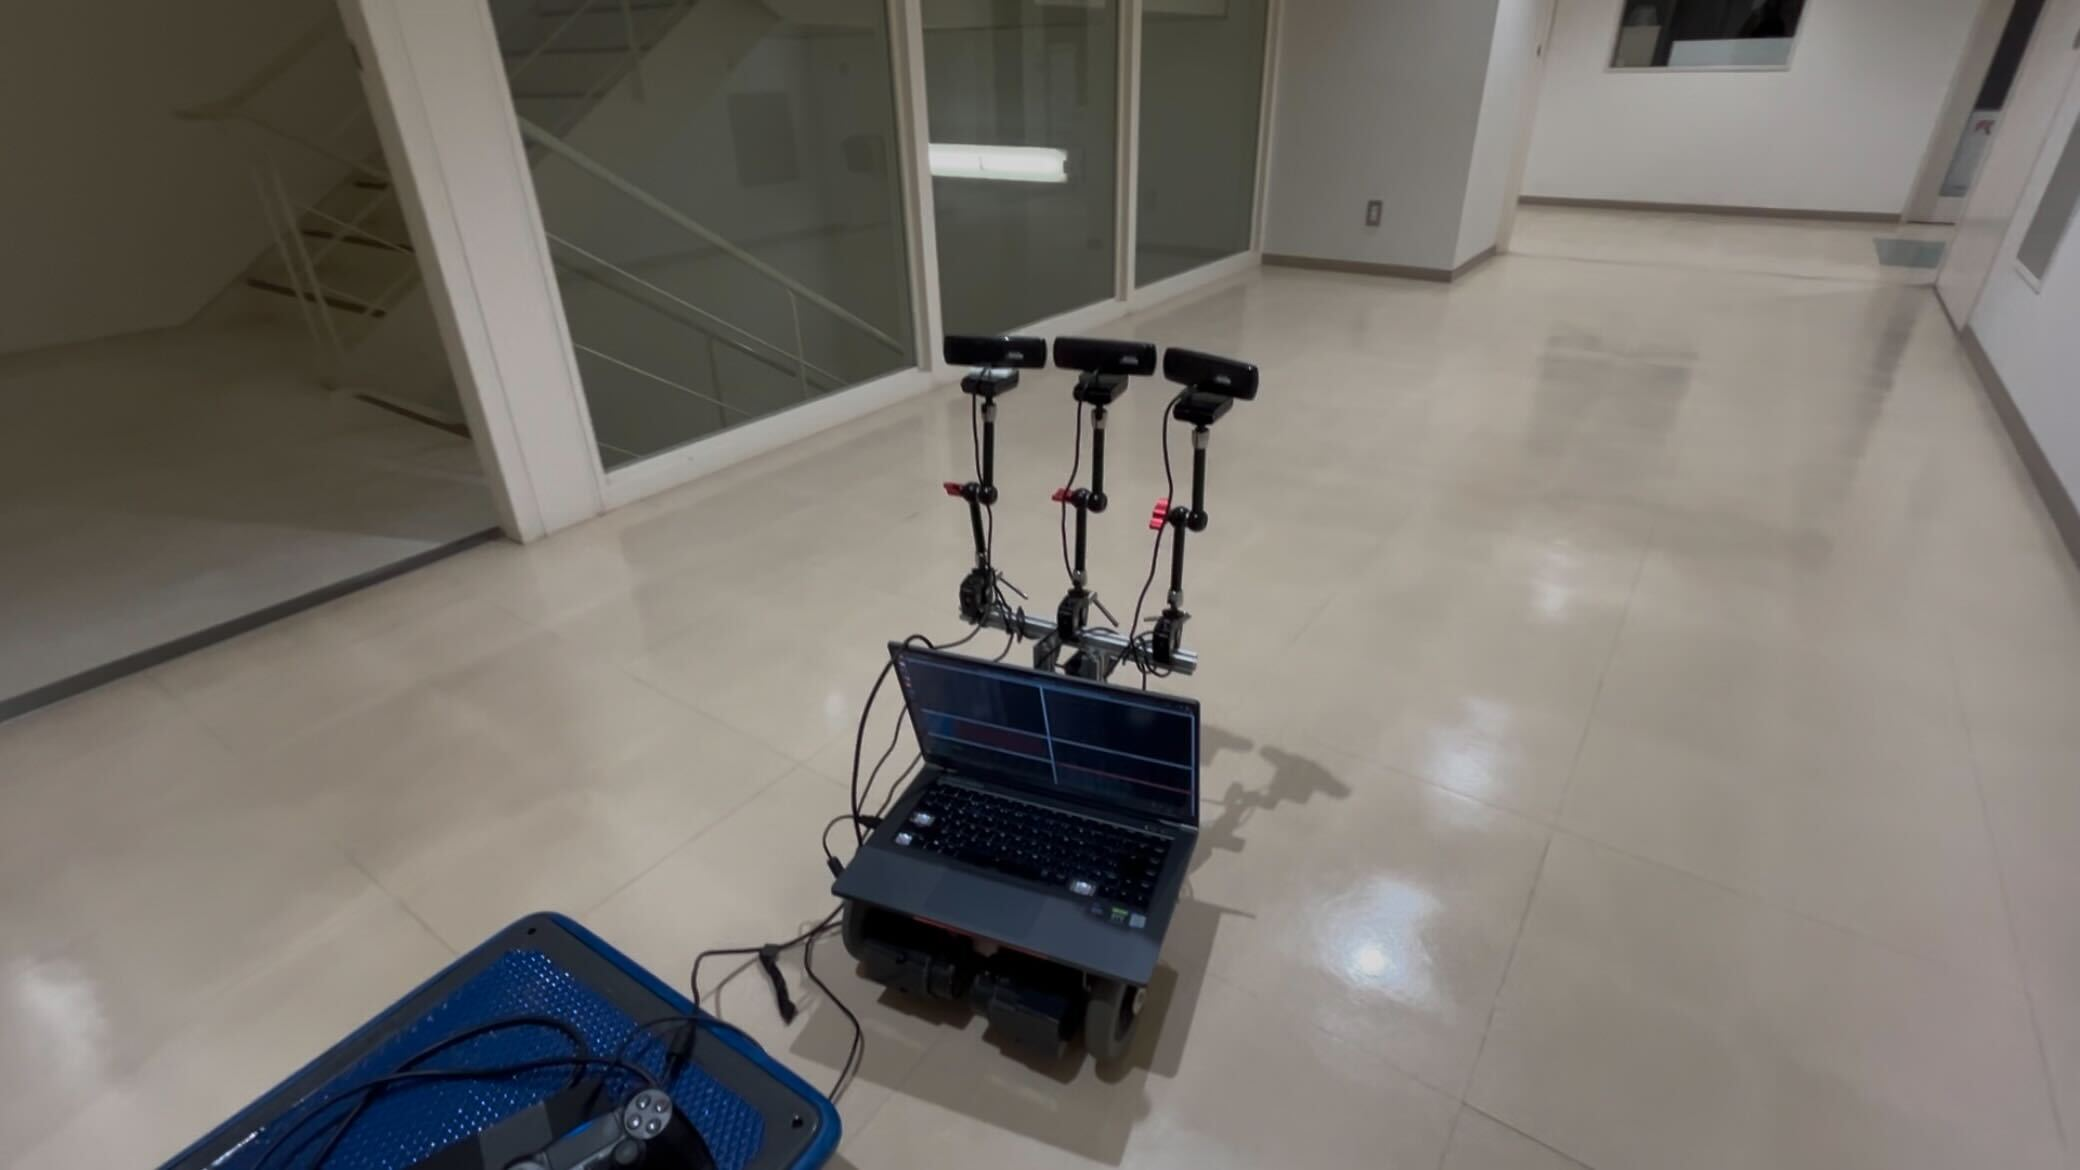
\includegraphics[keepaspectratio, width=70mm]{images/png/ishiguro/exp_8.png}
      % \subcaption{停止(End)}
        \end{minipage} &
        \begin{minipage}[t]{0.5\textwidth}
            \centering
            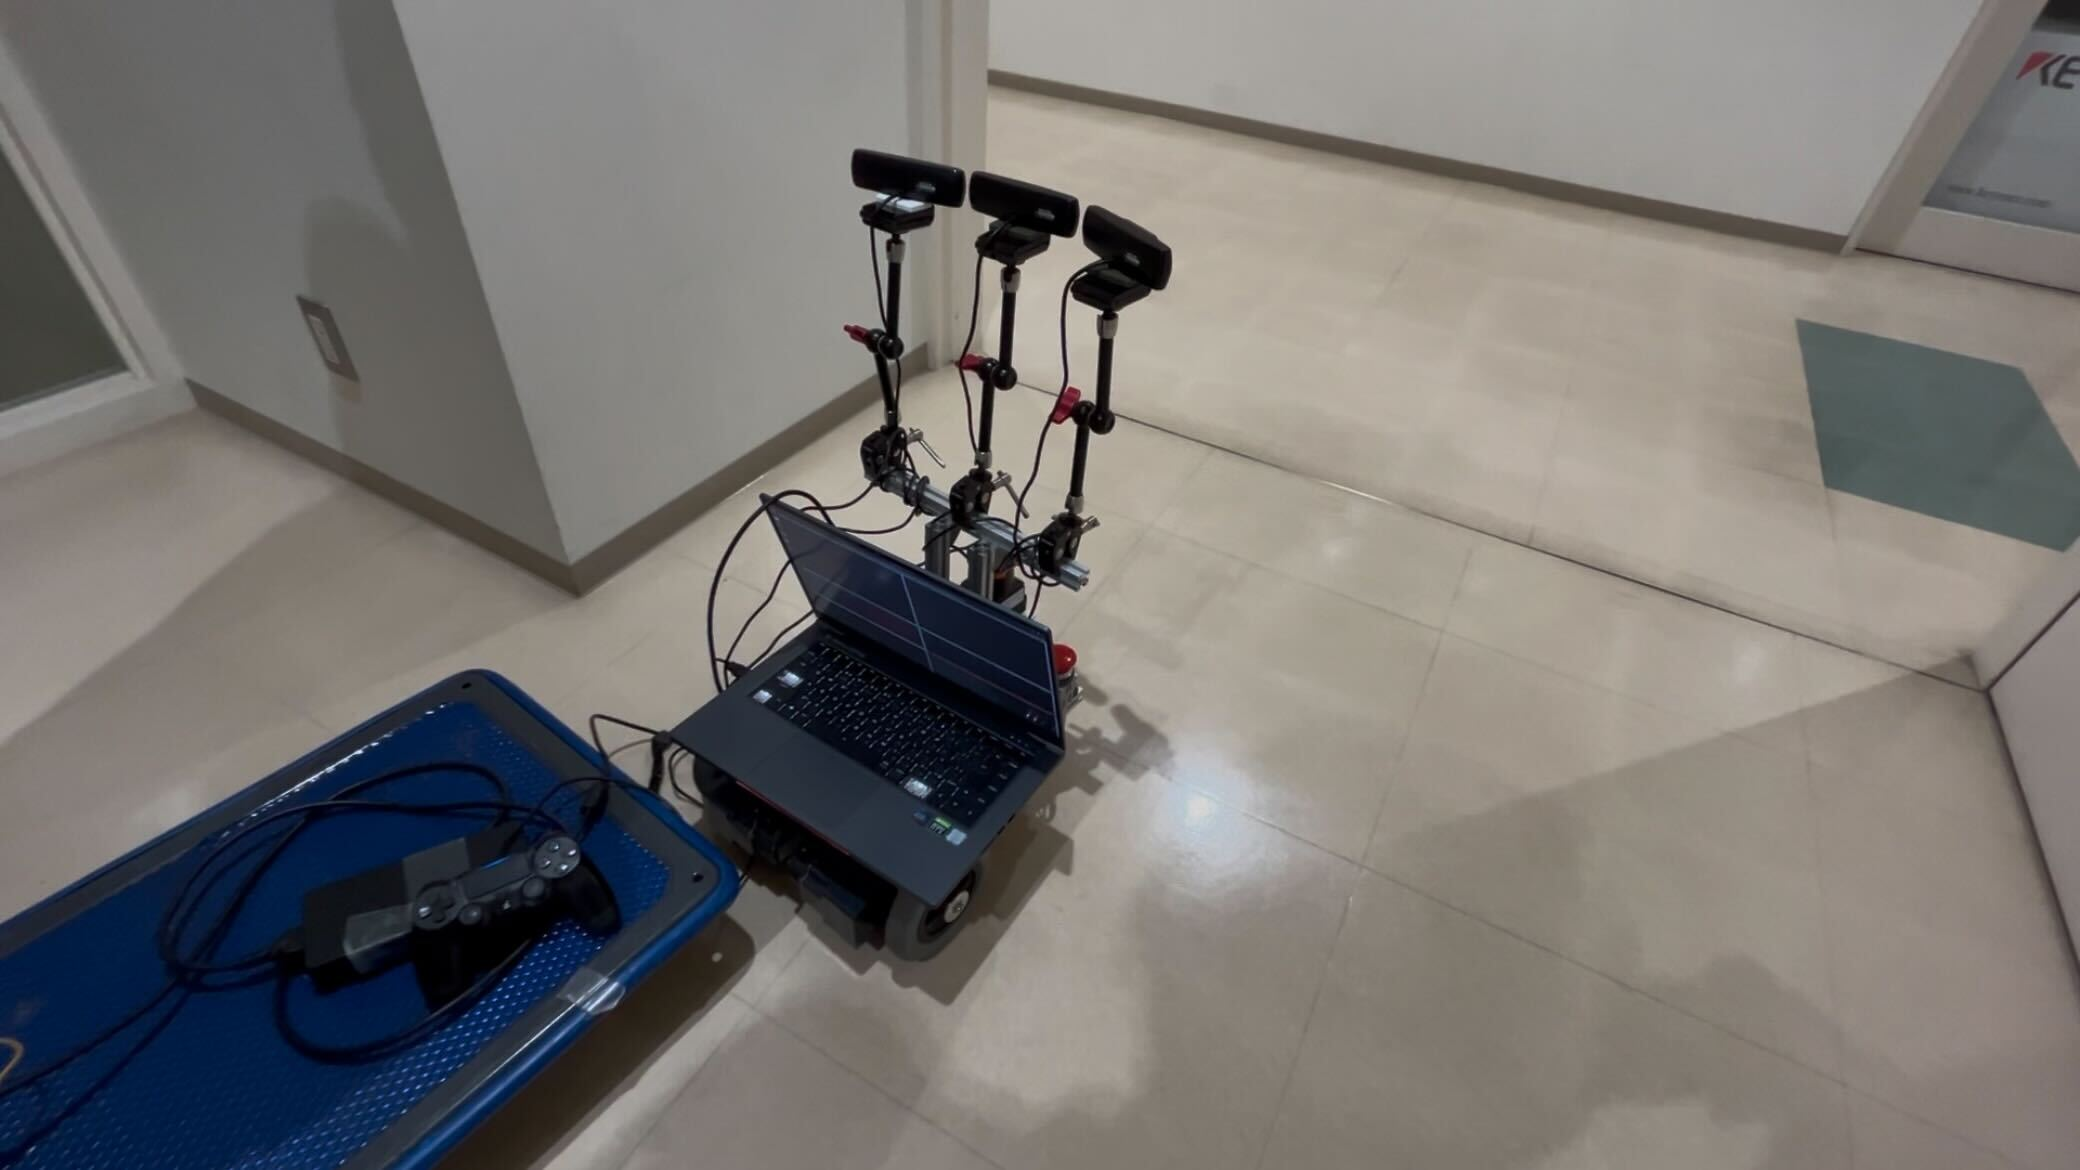
\includegraphics[keepaspectratio, width=70mm]{images/png/ishiguro/exp_9.png}
      % \subcaption{停止(End)}
        \end{minipage}
    \end{tabular}
\caption{An example of the robot applied the proposed system}
\label{fig:exp_path}
\end{figure*}

先行研究で走行が確認されていないエリアでも,ロボットがシナリオの道順に沿って,分岐路で適切な経路を選択する様子が確認できた.

失敗した4例ではそれぞれ,曲がり角で左折すべきところを直進した.
以下に失敗した箇所について示す.
失敗した箇所でも通路の特徴の分類は正しく行われており,経路追従モジュールに与えられる目標方向も正しい値が入力されていた.
一方で,通路分類の結果の切り替わりが遅いことを発見した.
以下〜〜に示す画像は学習時に「左折」の目標方向を与えたタイミングでのロボットの位置である.
〜〜に示す画像は,通路の分類が切り替わったタイミングで撮影したロボットの位置を表す.
このように分類遅れることで経路追従モジュールに目標方向が与えられるのが学習時より遅いことが確認できた.
確認として,学習時と同じタイミングで経路追従モジュールに目標方向を与えた場合,左折する様子が確認できた.
このことから,失敗要因として通路分類の切り替わりが遅いことが考えられる.
